
% Default to the notebook output style

    


% Inherit from the specified cell style.




    
\documentclass[11pt]{article}

    
    
    \usepackage[T1]{fontenc}
    % Nicer default font (+ math font) than Computer Modern for most use cases
    \usepackage{mathpazo}

    % Basic figure setup, for now with no caption control since it's done
    % automatically by Pandoc (which extracts ![](path) syntax from Markdown).
    \usepackage{graphicx}
    % We will generate all images so they have a width \maxwidth. This means
    % that they will get their normal width if they fit onto the page, but
    % are scaled down if they would overflow the margins.
    \makeatletter
    \def\maxwidth{\ifdim\Gin@nat@width>\linewidth\linewidth
    \else\Gin@nat@width\fi}
    \makeatother
    \let\Oldincludegraphics\includegraphics
    % Set max figure width to be 80% of text width, for now hardcoded.
    \renewcommand{\includegraphics}[1]{\Oldincludegraphics[width=.8\maxwidth]{#1}}
    % Ensure that by default, figures have no caption (until we provide a
    % proper Figure object with a Caption API and a way to capture that
    % in the conversion process - todo).
    \usepackage{caption}
    \DeclareCaptionLabelFormat{nolabel}{}
    \captionsetup{labelformat=nolabel}

    \usepackage{adjustbox} % Used to constrain images to a maximum size 
    \usepackage{xcolor} % Allow colors to be defined
    \usepackage{enumerate} % Needed for markdown enumerations to work
    \usepackage{geometry} % Used to adjust the document margins
    \usepackage{amsmath} % Equations
    \usepackage{amssymb} % Equations
    \usepackage{textcomp} % defines textquotesingle
    % Hack from http://tex.stackexchange.com/a/47451/13684:
    \AtBeginDocument{%
        \def\PYZsq{\textquotesingle}% Upright quotes in Pygmentized code
    }
    \usepackage{upquote} % Upright quotes for verbatim code
    \usepackage{eurosym} % defines \euro
    \usepackage[mathletters]{ucs} % Extended unicode (utf-8) support
    \usepackage[utf8x]{inputenc} % Allow utf-8 characters in the tex document
    \usepackage{fancyvrb} % verbatim replacement that allows latex
    \usepackage{grffile} % extends the file name processing of package graphics 
                         % to support a larger range 
    % The hyperref package gives us a pdf with properly built
    % internal navigation ('pdf bookmarks' for the table of contents,
    % internal cross-reference links, web links for URLs, etc.)
    \usepackage{hyperref}
    \usepackage{longtable} % longtable support required by pandoc >1.10
    \usepackage{booktabs}  % table support for pandoc > 1.12.2
    \usepackage[inline]{enumitem} % IRkernel/repr support (it uses the enumerate* environment)
    \usepackage[normalem]{ulem} % ulem is needed to support strikethroughs (\sout)
                                % normalem makes italics be italics, not underlines
    

    
    
    % Colors for the hyperref package
    \definecolor{urlcolor}{rgb}{0,.145,.698}
    \definecolor{linkcolor}{rgb}{.71,0.21,0.01}
    \definecolor{citecolor}{rgb}{.12,.54,.11}

    % ANSI colors
    \definecolor{ansi-black}{HTML}{3E424D}
    \definecolor{ansi-black-intense}{HTML}{282C36}
    \definecolor{ansi-red}{HTML}{E75C58}
    \definecolor{ansi-red-intense}{HTML}{B22B31}
    \definecolor{ansi-green}{HTML}{00A250}
    \definecolor{ansi-green-intense}{HTML}{007427}
    \definecolor{ansi-yellow}{HTML}{DDB62B}
    \definecolor{ansi-yellow-intense}{HTML}{B27D12}
    \definecolor{ansi-blue}{HTML}{208FFB}
    \definecolor{ansi-blue-intense}{HTML}{0065CA}
    \definecolor{ansi-magenta}{HTML}{D160C4}
    \definecolor{ansi-magenta-intense}{HTML}{A03196}
    \definecolor{ansi-cyan}{HTML}{60C6C8}
    \definecolor{ansi-cyan-intense}{HTML}{258F8F}
    \definecolor{ansi-white}{HTML}{C5C1B4}
    \definecolor{ansi-white-intense}{HTML}{A1A6B2}

    % commands and environments needed by pandoc snippets
    % extracted from the output of `pandoc -s`
    \providecommand{\tightlist}{%
      \setlength{\itemsep}{0pt}\setlength{\parskip}{0pt}}
    \DefineVerbatimEnvironment{Highlighting}{Verbatim}{commandchars=\\\{\}}
    % Add ',fontsize=\small' for more characters per line
    \newenvironment{Shaded}{}{}
    \newcommand{\KeywordTok}[1]{\textcolor[rgb]{0.00,0.44,0.13}{\textbf{{#1}}}}
    \newcommand{\DataTypeTok}[1]{\textcolor[rgb]{0.56,0.13,0.00}{{#1}}}
    \newcommand{\DecValTok}[1]{\textcolor[rgb]{0.25,0.63,0.44}{{#1}}}
    \newcommand{\BaseNTok}[1]{\textcolor[rgb]{0.25,0.63,0.44}{{#1}}}
    \newcommand{\FloatTok}[1]{\textcolor[rgb]{0.25,0.63,0.44}{{#1}}}
    \newcommand{\CharTok}[1]{\textcolor[rgb]{0.25,0.44,0.63}{{#1}}}
    \newcommand{\StringTok}[1]{\textcolor[rgb]{0.25,0.44,0.63}{{#1}}}
    \newcommand{\CommentTok}[1]{\textcolor[rgb]{0.38,0.63,0.69}{\textit{{#1}}}}
    \newcommand{\OtherTok}[1]{\textcolor[rgb]{0.00,0.44,0.13}{{#1}}}
    \newcommand{\AlertTok}[1]{\textcolor[rgb]{1.00,0.00,0.00}{\textbf{{#1}}}}
    \newcommand{\FunctionTok}[1]{\textcolor[rgb]{0.02,0.16,0.49}{{#1}}}
    \newcommand{\RegionMarkerTok}[1]{{#1}}
    \newcommand{\ErrorTok}[1]{\textcolor[rgb]{1.00,0.00,0.00}{\textbf{{#1}}}}
    \newcommand{\NormalTok}[1]{{#1}}
    
    % Additional commands for more recent versions of Pandoc
    \newcommand{\ConstantTok}[1]{\textcolor[rgb]{0.53,0.00,0.00}{{#1}}}
    \newcommand{\SpecialCharTok}[1]{\textcolor[rgb]{0.25,0.44,0.63}{{#1}}}
    \newcommand{\VerbatimStringTok}[1]{\textcolor[rgb]{0.25,0.44,0.63}{{#1}}}
    \newcommand{\SpecialStringTok}[1]{\textcolor[rgb]{0.73,0.40,0.53}{{#1}}}
    \newcommand{\ImportTok}[1]{{#1}}
    \newcommand{\DocumentationTok}[1]{\textcolor[rgb]{0.73,0.13,0.13}{\textit{{#1}}}}
    \newcommand{\AnnotationTok}[1]{\textcolor[rgb]{0.38,0.63,0.69}{\textbf{\textit{{#1}}}}}
    \newcommand{\CommentVarTok}[1]{\textcolor[rgb]{0.38,0.63,0.69}{\textbf{\textit{{#1}}}}}
    \newcommand{\VariableTok}[1]{\textcolor[rgb]{0.10,0.09,0.49}{{#1}}}
    \newcommand{\ControlFlowTok}[1]{\textcolor[rgb]{0.00,0.44,0.13}{\textbf{{#1}}}}
    \newcommand{\OperatorTok}[1]{\textcolor[rgb]{0.40,0.40,0.40}{{#1}}}
    \newcommand{\BuiltInTok}[1]{{#1}}
    \newcommand{\ExtensionTok}[1]{{#1}}
    \newcommand{\PreprocessorTok}[1]{\textcolor[rgb]{0.74,0.48,0.00}{{#1}}}
    \newcommand{\AttributeTok}[1]{\textcolor[rgb]{0.49,0.56,0.16}{{#1}}}
    \newcommand{\InformationTok}[1]{\textcolor[rgb]{0.38,0.63,0.69}{\textbf{\textit{{#1}}}}}
    \newcommand{\WarningTok}[1]{\textcolor[rgb]{0.38,0.63,0.69}{\textbf{\textit{{#1}}}}}
    
    
    % Define a nice break command that doesn't care if a line doesn't already
    % exist.
    \def\br{\hspace*{\fill} \\* }
    % Math Jax compatability definitions
    \def\gt{>}
    \def\lt{<}
    % Document parameters
    \title{N170 Emotiv Exploratory}
    
    
    

    % Pygments definitions
    
\makeatletter
\def\PY@reset{\let\PY@it=\relax \let\PY@bf=\relax%
    \let\PY@ul=\relax \let\PY@tc=\relax%
    \let\PY@bc=\relax \let\PY@ff=\relax}
\def\PY@tok#1{\csname PY@tok@#1\endcsname}
\def\PY@toks#1+{\ifx\relax#1\empty\else%
    \PY@tok{#1}\expandafter\PY@toks\fi}
\def\PY@do#1{\PY@bc{\PY@tc{\PY@ul{%
    \PY@it{\PY@bf{\PY@ff{#1}}}}}}}
\def\PY#1#2{\PY@reset\PY@toks#1+\relax+\PY@do{#2}}

\expandafter\def\csname PY@tok@sh\endcsname{\def\PY@tc##1{\textcolor[rgb]{0.73,0.13,0.13}{##1}}}
\expandafter\def\csname PY@tok@go\endcsname{\def\PY@tc##1{\textcolor[rgb]{0.53,0.53,0.53}{##1}}}
\expandafter\def\csname PY@tok@nd\endcsname{\def\PY@tc##1{\textcolor[rgb]{0.67,0.13,1.00}{##1}}}
\expandafter\def\csname PY@tok@cm\endcsname{\let\PY@it=\textit\def\PY@tc##1{\textcolor[rgb]{0.25,0.50,0.50}{##1}}}
\expandafter\def\csname PY@tok@mi\endcsname{\def\PY@tc##1{\textcolor[rgb]{0.40,0.40,0.40}{##1}}}
\expandafter\def\csname PY@tok@s1\endcsname{\def\PY@tc##1{\textcolor[rgb]{0.73,0.13,0.13}{##1}}}
\expandafter\def\csname PY@tok@cp\endcsname{\def\PY@tc##1{\textcolor[rgb]{0.74,0.48,0.00}{##1}}}
\expandafter\def\csname PY@tok@k\endcsname{\let\PY@bf=\textbf\def\PY@tc##1{\textcolor[rgb]{0.00,0.50,0.00}{##1}}}
\expandafter\def\csname PY@tok@no\endcsname{\def\PY@tc##1{\textcolor[rgb]{0.53,0.00,0.00}{##1}}}
\expandafter\def\csname PY@tok@kn\endcsname{\let\PY@bf=\textbf\def\PY@tc##1{\textcolor[rgb]{0.00,0.50,0.00}{##1}}}
\expandafter\def\csname PY@tok@s\endcsname{\def\PY@tc##1{\textcolor[rgb]{0.73,0.13,0.13}{##1}}}
\expandafter\def\csname PY@tok@vi\endcsname{\def\PY@tc##1{\textcolor[rgb]{0.10,0.09,0.49}{##1}}}
\expandafter\def\csname PY@tok@sc\endcsname{\def\PY@tc##1{\textcolor[rgb]{0.73,0.13,0.13}{##1}}}
\expandafter\def\csname PY@tok@ow\endcsname{\let\PY@bf=\textbf\def\PY@tc##1{\textcolor[rgb]{0.67,0.13,1.00}{##1}}}
\expandafter\def\csname PY@tok@kd\endcsname{\let\PY@bf=\textbf\def\PY@tc##1{\textcolor[rgb]{0.00,0.50,0.00}{##1}}}
\expandafter\def\csname PY@tok@gs\endcsname{\let\PY@bf=\textbf}
\expandafter\def\csname PY@tok@kp\endcsname{\def\PY@tc##1{\textcolor[rgb]{0.00,0.50,0.00}{##1}}}
\expandafter\def\csname PY@tok@dl\endcsname{\def\PY@tc##1{\textcolor[rgb]{0.73,0.13,0.13}{##1}}}
\expandafter\def\csname PY@tok@bp\endcsname{\def\PY@tc##1{\textcolor[rgb]{0.00,0.50,0.00}{##1}}}
\expandafter\def\csname PY@tok@nb\endcsname{\def\PY@tc##1{\textcolor[rgb]{0.00,0.50,0.00}{##1}}}
\expandafter\def\csname PY@tok@il\endcsname{\def\PY@tc##1{\textcolor[rgb]{0.40,0.40,0.40}{##1}}}
\expandafter\def\csname PY@tok@na\endcsname{\def\PY@tc##1{\textcolor[rgb]{0.49,0.56,0.16}{##1}}}
\expandafter\def\csname PY@tok@m\endcsname{\def\PY@tc##1{\textcolor[rgb]{0.40,0.40,0.40}{##1}}}
\expandafter\def\csname PY@tok@mo\endcsname{\def\PY@tc##1{\textcolor[rgb]{0.40,0.40,0.40}{##1}}}
\expandafter\def\csname PY@tok@kt\endcsname{\def\PY@tc##1{\textcolor[rgb]{0.69,0.00,0.25}{##1}}}
\expandafter\def\csname PY@tok@gt\endcsname{\def\PY@tc##1{\textcolor[rgb]{0.00,0.27,0.87}{##1}}}
\expandafter\def\csname PY@tok@c1\endcsname{\let\PY@it=\textit\def\PY@tc##1{\textcolor[rgb]{0.25,0.50,0.50}{##1}}}
\expandafter\def\csname PY@tok@ne\endcsname{\let\PY@bf=\textbf\def\PY@tc##1{\textcolor[rgb]{0.82,0.25,0.23}{##1}}}
\expandafter\def\csname PY@tok@kc\endcsname{\let\PY@bf=\textbf\def\PY@tc##1{\textcolor[rgb]{0.00,0.50,0.00}{##1}}}
\expandafter\def\csname PY@tok@w\endcsname{\def\PY@tc##1{\textcolor[rgb]{0.73,0.73,0.73}{##1}}}
\expandafter\def\csname PY@tok@o\endcsname{\def\PY@tc##1{\textcolor[rgb]{0.40,0.40,0.40}{##1}}}
\expandafter\def\csname PY@tok@vm\endcsname{\def\PY@tc##1{\textcolor[rgb]{0.10,0.09,0.49}{##1}}}
\expandafter\def\csname PY@tok@err\endcsname{\def\PY@bc##1{\setlength{\fboxsep}{0pt}\fcolorbox[rgb]{1.00,0.00,0.00}{1,1,1}{\strut ##1}}}
\expandafter\def\csname PY@tok@nc\endcsname{\let\PY@bf=\textbf\def\PY@tc##1{\textcolor[rgb]{0.00,0.00,1.00}{##1}}}
\expandafter\def\csname PY@tok@sd\endcsname{\let\PY@it=\textit\def\PY@tc##1{\textcolor[rgb]{0.73,0.13,0.13}{##1}}}
\expandafter\def\csname PY@tok@mh\endcsname{\def\PY@tc##1{\textcolor[rgb]{0.40,0.40,0.40}{##1}}}
\expandafter\def\csname PY@tok@nn\endcsname{\let\PY@bf=\textbf\def\PY@tc##1{\textcolor[rgb]{0.00,0.00,1.00}{##1}}}
\expandafter\def\csname PY@tok@si\endcsname{\let\PY@bf=\textbf\def\PY@tc##1{\textcolor[rgb]{0.73,0.40,0.53}{##1}}}
\expandafter\def\csname PY@tok@gd\endcsname{\def\PY@tc##1{\textcolor[rgb]{0.63,0.00,0.00}{##1}}}
\expandafter\def\csname PY@tok@mf\endcsname{\def\PY@tc##1{\textcolor[rgb]{0.40,0.40,0.40}{##1}}}
\expandafter\def\csname PY@tok@vc\endcsname{\def\PY@tc##1{\textcolor[rgb]{0.10,0.09,0.49}{##1}}}
\expandafter\def\csname PY@tok@sr\endcsname{\def\PY@tc##1{\textcolor[rgb]{0.73,0.40,0.53}{##1}}}
\expandafter\def\csname PY@tok@gh\endcsname{\let\PY@bf=\textbf\def\PY@tc##1{\textcolor[rgb]{0.00,0.00,0.50}{##1}}}
\expandafter\def\csname PY@tok@ch\endcsname{\let\PY@it=\textit\def\PY@tc##1{\textcolor[rgb]{0.25,0.50,0.50}{##1}}}
\expandafter\def\csname PY@tok@nl\endcsname{\def\PY@tc##1{\textcolor[rgb]{0.63,0.63,0.00}{##1}}}
\expandafter\def\csname PY@tok@cpf\endcsname{\let\PY@it=\textit\def\PY@tc##1{\textcolor[rgb]{0.25,0.50,0.50}{##1}}}
\expandafter\def\csname PY@tok@gr\endcsname{\def\PY@tc##1{\textcolor[rgb]{1.00,0.00,0.00}{##1}}}
\expandafter\def\csname PY@tok@ss\endcsname{\def\PY@tc##1{\textcolor[rgb]{0.10,0.09,0.49}{##1}}}
\expandafter\def\csname PY@tok@se\endcsname{\let\PY@bf=\textbf\def\PY@tc##1{\textcolor[rgb]{0.73,0.40,0.13}{##1}}}
\expandafter\def\csname PY@tok@c\endcsname{\let\PY@it=\textit\def\PY@tc##1{\textcolor[rgb]{0.25,0.50,0.50}{##1}}}
\expandafter\def\csname PY@tok@nf\endcsname{\def\PY@tc##1{\textcolor[rgb]{0.00,0.00,1.00}{##1}}}
\expandafter\def\csname PY@tok@nt\endcsname{\let\PY@bf=\textbf\def\PY@tc##1{\textcolor[rgb]{0.00,0.50,0.00}{##1}}}
\expandafter\def\csname PY@tok@ge\endcsname{\let\PY@it=\textit}
\expandafter\def\csname PY@tok@sb\endcsname{\def\PY@tc##1{\textcolor[rgb]{0.73,0.13,0.13}{##1}}}
\expandafter\def\csname PY@tok@fm\endcsname{\def\PY@tc##1{\textcolor[rgb]{0.00,0.00,1.00}{##1}}}
\expandafter\def\csname PY@tok@gp\endcsname{\let\PY@bf=\textbf\def\PY@tc##1{\textcolor[rgb]{0.00,0.00,0.50}{##1}}}
\expandafter\def\csname PY@tok@gu\endcsname{\let\PY@bf=\textbf\def\PY@tc##1{\textcolor[rgb]{0.50,0.00,0.50}{##1}}}
\expandafter\def\csname PY@tok@cs\endcsname{\let\PY@it=\textit\def\PY@tc##1{\textcolor[rgb]{0.25,0.50,0.50}{##1}}}
\expandafter\def\csname PY@tok@vg\endcsname{\def\PY@tc##1{\textcolor[rgb]{0.10,0.09,0.49}{##1}}}
\expandafter\def\csname PY@tok@sa\endcsname{\def\PY@tc##1{\textcolor[rgb]{0.73,0.13,0.13}{##1}}}
\expandafter\def\csname PY@tok@nv\endcsname{\def\PY@tc##1{\textcolor[rgb]{0.10,0.09,0.49}{##1}}}
\expandafter\def\csname PY@tok@kr\endcsname{\let\PY@bf=\textbf\def\PY@tc##1{\textcolor[rgb]{0.00,0.50,0.00}{##1}}}
\expandafter\def\csname PY@tok@mb\endcsname{\def\PY@tc##1{\textcolor[rgb]{0.40,0.40,0.40}{##1}}}
\expandafter\def\csname PY@tok@sx\endcsname{\def\PY@tc##1{\textcolor[rgb]{0.00,0.50,0.00}{##1}}}
\expandafter\def\csname PY@tok@ni\endcsname{\let\PY@bf=\textbf\def\PY@tc##1{\textcolor[rgb]{0.60,0.60,0.60}{##1}}}
\expandafter\def\csname PY@tok@gi\endcsname{\def\PY@tc##1{\textcolor[rgb]{0.00,0.63,0.00}{##1}}}
\expandafter\def\csname PY@tok@s2\endcsname{\def\PY@tc##1{\textcolor[rgb]{0.73,0.13,0.13}{##1}}}

\def\PYZbs{\char`\\}
\def\PYZus{\char`\_}
\def\PYZob{\char`\{}
\def\PYZcb{\char`\}}
\def\PYZca{\char`\^}
\def\PYZam{\char`\&}
\def\PYZlt{\char`\<}
\def\PYZgt{\char`\>}
\def\PYZsh{\char`\#}
\def\PYZpc{\char`\%}
\def\PYZdl{\char`\$}
\def\PYZhy{\char`\-}
\def\PYZsq{\char`\'}
\def\PYZdq{\char`\"}
\def\PYZti{\char`\~}
% for compatibility with earlier versions
\def\PYZat{@}
\def\PYZlb{[}
\def\PYZrb{]}
\makeatother


    % Exact colors from NB
    \definecolor{incolor}{rgb}{0.0, 0.0, 0.5}
    \definecolor{outcolor}{rgb}{0.545, 0.0, 0.0}



    
    % Prevent overflowing lines due to hard-to-break entities
    \sloppy 
    % Setup hyperref package
    \hypersetup{
      breaklinks=true,  % so long urls are correctly broken across lines
      colorlinks=true,
      urlcolor=urlcolor,
      linkcolor=linkcolor,
      citecolor=citecolor,
      }
    % Slightly bigger margins than the latex defaults
    
    \geometry{verbose,tmargin=1in,bmargin=1in,lmargin=1in,rmargin=1in}
    
    

    \begin{document}
    
    
    \maketitle
    
    

    
    \section{Emotiv EEG Data Visualization
Options}\label{emotiv-eeg-data-visualization-options}

A short overview of what's possible with the MNE library and what we
should focus on including into the first iteration of the BrainWaves
app.

    \begin{Verbatim}[commandchars=\\\{\}]
{\color{incolor}In [{\color{incolor}220}]:} \PY{k+kn}{from} \PY{n+nn}{mne} \PY{k}{import} \PY{n}{Epochs}\PY{p}{,} \PY{n}{find\PYZus{}events}\PY{p}{,} \PY{n}{set\PYZus{}eeg\PYZus{}reference}\PY{p}{,} \PY{n}{read\PYZus{}epochs}\PY{p}{,} \PY{n}{viz}\PY{p}{,} \PY{n}{combine\PYZus{}evoked}
          \PY{k+kn}{from} \PY{n+nn}{time} \PY{k}{import} \PY{n}{time}\PY{p}{,} \PY{n}{strftime}\PY{p}{,} \PY{n}{gmtime}
          \PY{k+kn}{from} \PY{n+nn}{collections} \PY{k}{import} \PY{n}{OrderedDict}
          \PY{k+kn}{from} \PY{n+nn}{glob} \PY{k}{import} \PY{n}{glob}
          \PY{k+kn}{from} \PY{n+nn}{collections} \PY{k}{import} \PY{n}{OrderedDict}
          \PY{k+kn}{from} \PY{n+nn}{mne} \PY{k}{import} \PY{n}{create\PYZus{}info}\PY{p}{,} \PY{n}{concatenate\PYZus{}raws}
          \PY{k+kn}{from} \PY{n+nn}{mne}\PY{n+nn}{.}\PY{n+nn}{io} \PY{k}{import} \PY{n}{RawArray}
          \PY{k+kn}{from} \PY{n+nn}{mne}\PY{n+nn}{.}\PY{n+nn}{channels} \PY{k}{import} \PY{n}{read\PYZus{}montage}
          \PY{k+kn}{import} \PY{n+nn}{pandas} \PY{k}{as} \PY{n+nn}{pd}
          \PY{k+kn}{import} \PY{n+nn}{numpy} \PY{k}{as} \PY{n+nn}{np}
          \PY{k+kn}{import} \PY{n+nn}{seaborn} \PY{k}{as} \PY{n+nn}{sns}
          \PY{k+kn}{import} \PY{n+nn}{matplotlib}\PY{n+nn}{.}\PY{n+nn}{pyplot} \PY{k}{as} \PY{n+nn}{plt}
          \PY{k+kn}{import} \PY{n+nn}{sys}\PY{o}{,} \PY{n+nn}{os}
          \PY{n}{sys}\PY{o}{.}\PY{n}{path}\PY{o}{.}\PY{n}{append}\PY{p}{(}\PY{n}{os}\PY{o}{.}\PY{n}{path}\PY{o}{.}\PY{n}{join}\PY{p}{(}\PY{n}{os}\PY{o}{.}\PY{n}{path}\PY{o}{.}\PY{n}{dirname}\PY{p}{(}\PY{n}{os}\PY{o}{.}\PY{n}{getcwd}\PY{p}{(}\PY{p}{)}\PY{p}{)}\PY{p}{,} \PY{l+s+s1}{\PYZsq{}}\PY{l+s+s1}{app}\PY{l+s+s1}{\PYZsq{}}\PY{p}{,}\PY{l+s+s1}{\PYZsq{}}\PY{l+s+s1}{utils}\PY{l+s+s1}{\PYZsq{}}\PY{p}{,}\PY{l+s+s1}{\PYZsq{}}\PY{l+s+s1}{jupyter}\PY{l+s+s1}{\PYZsq{}}\PY{p}{)}\PY{p}{)}
          \PY{k+kn}{import} \PY{n+nn}{utils}
          \PY{o}{\PYZpc{}}\PY{k}{matplotlib} inline
          \PY{k+kn}{import} \PY{n+nn}{warnings}
          \PY{n}{warnings}\PY{o}{.}\PY{n}{filterwarnings}\PY{p}{(}\PY{l+s+s2}{\PYZdq{}}\PY{l+s+s2}{ignore}\PY{l+s+s2}{\PYZdq{}}\PY{p}{)}
\end{Verbatim}


    This is a dataset that has been collected and cleaned in the app. It is
comprised of two 2-minute runs of the Faces Houses experiment and,
although it doesn't show a classic N170, there is some interesting
event-related potential information in the data. It actually looks like
there may be P300s.

    \begin{Verbatim}[commandchars=\\\{\}]
{\color{incolor}In [{\color{incolor}182}]:} \PY{n}{epochs} \PY{o}{=} \PY{n}{read\PYZus{}epochs}\PY{p}{(}\PY{l+s+s1}{\PYZsq{}}\PY{l+s+s1}{/home/dano/BrainWaves Workspaces/Dano Nelson Faces Houses/Data/Subash\PYZus{}2\PYZhy{}epo.fif}\PY{l+s+s1}{\PYZsq{}}\PY{p}{)}
          \PY{n}{face\PYZus{}epochs} \PY{o}{=} \PY{n}{epochs}\PY{p}{[}\PY{l+s+s1}{\PYZsq{}}\PY{l+s+s1}{Face}\PY{l+s+s1}{\PYZsq{}}\PY{p}{]}
          \PY{n}{house\PYZus{}epochs} \PY{o}{=} \PY{n}{epochs}\PY{p}{[}\PY{l+s+s1}{\PYZsq{}}\PY{l+s+s1}{House}\PY{l+s+s1}{\PYZsq{}}\PY{p}{]}
\end{Verbatim}


    \begin{Verbatim}[commandchars=\\\{\}]
Reading /home/dano/BrainWaves Workspaces/Dano Nelson Faces Houses/Data/Subash\_2-epo.fif {\ldots}
    Found the data of interest:
        t =    -101.56 {\ldots}     796.88 ms
        0 CTF compensation matrices available
157 matching events found
Applying baseline correction (mode: mean)
157 matching events found
Applying baseline correction (mode: mean)
Not setting metadata
0 projection items activated

    \end{Verbatim}

    \begin{Verbatim}[commandchars=\\\{\}]
{\color{incolor}In [{\color{incolor}183}]:} \PY{o}{\PYZpc{}}\PY{k}{matplotlib} inline
          \PY{k+kn}{import} \PY{n+nn}{numpy} \PY{k}{as} \PY{n+nn}{np}
          \PY{k+kn}{import} \PY{n+nn}{matplotlib}\PY{n+nn}{.}\PY{n+nn}{pyplot} \PY{k}{as} \PY{n+nn}{plt}
          \PY{k+kn}{from} \PY{n+nn}{mne}\PY{n+nn}{.}\PY{n+nn}{datasets} \PY{k}{import} \PY{n}{sample}
          \PY{k+kn}{from} \PY{n+nn}{mne} \PY{k}{import} \PY{n}{read\PYZus{}evokeds}
          
          \PY{n}{house\PYZus{}evoked} \PY{o}{=} \PY{n}{house\PYZus{}epochs}\PY{o}{.}\PY{n}{average}\PY{p}{(}\PY{p}{)}
          \PY{n}{face\PYZus{}evoked} \PY{o}{=} \PY{n}{face\PYZus{}epochs}\PY{o}{.}\PY{n}{average}\PY{p}{(}\PY{p}{)}
\end{Verbatim}


    The way I see it, the students have to demonstrate that they can make
three types of comparisons on this screen: comparing between conditions
(faces and house, etc.), comparing between channels, and comparing
between subjects. This gets a bit complicated because the comparisons
between channels and subjects should really be based on the
\emph{difference between conditions that they've found by comparing
between conditions}

I've broken up the different visualizations into these different 'jobs'.
I'm not sure which order these tasks should necessarily be completed,
but I'm putting them in the order that makes most sense for how I would
explore a dataset.

\section{Job 1: Comparing Between
Conditions}\label{job-1-comparing-between-conditions}

    \subsection{Averaged Epoch Difference
Plot}\label{averaged-epoch-difference-plot}

This is our standard, which is good at showing differences between
conditions with statistical significance indicated by the colored
background confidence interval.

However, it kind of sucks because it only displays one channel at a time

    \begin{Verbatim}[commandchars=\\\{\}]
{\color{incolor}In [{\color{incolor}197}]:} \PY{c+c1}{\PYZsh{} Computation}
          \PY{n}{conditions} \PY{o}{=} \PY{n}{OrderedDict}\PY{p}{(}\PY{p}{\PYZob{}}\PY{n}{key}\PY{p}{:} \PY{p}{[}\PY{n}{value}\PY{p}{]} \PY{k}{for} \PY{p}{(}\PY{n}{key}\PY{p}{,} \PY{n}{value}\PY{p}{)} \PY{o+ow}{in} \PY{n}{event\PYZus{}id}\PY{o}{.}\PY{n}{items}\PY{p}{(}\PY{p}{)}\PY{p}{\PYZcb{}}\PY{p}{)}
          
          \PY{c+c1}{\PYZsh{} Output}
          \PY{n}{X}\PY{p}{,} \PY{n}{y} \PY{o}{=} \PY{n}{utils}\PY{o}{.}\PY{n}{plot\PYZus{}conditions}\PY{p}{(}\PY{n}{epochs}\PY{p}{,} \PY{n}{ch\PYZus{}ind}\PY{o}{=}\PY{l+m+mi}{4}\PY{p}{,} \PY{n}{conditions}\PY{o}{=}\PY{n}{conditions}\PY{p}{,} 
                                          \PY{n}{ci}\PY{o}{=}\PY{l+m+mf}{97.5}\PY{p}{,} \PY{n}{n\PYZus{}boot}\PY{o}{=}\PY{l+m+mi}{1000}\PY{p}{,} \PY{n}{title}\PY{o}{=}\PY{l+s+s1}{\PYZsq{}}\PY{l+s+s1}{\PYZsq{}}\PY{p}{,} \PY{n}{diff\PYZus{}waveform}\PY{o}{=}\PY{k+kc}{None}\PY{p}{)}
\end{Verbatim}


    \begin{center}
    \adjustimage{max size={0.9\linewidth}{0.9\paperheight}}{output_7_0.png}
    \end{center}
    { \hspace*{\fill} \\}
    
    \subsection{Epochs Spectrogram}\label{epochs-spectrogram}

This is the first new interesting viz we could consider using. The
colors correspond to the amplitude of the EEG, with red being positive
and blue being negative. The epochs are all lined up in rows on the y
axis and ERPs should be visible as vertical colored bands.

Unfortunately, here we also can only view one plot at a time

    \begin{Verbatim}[commandchars=\\\{\}]
{\color{incolor}In [{\color{incolor}185}]:} \PY{n}{face\PYZus{}epochs}\PY{o}{.}\PY{n}{plot\PYZus{}image}\PY{p}{(}\PY{n}{title}\PY{o}{=}\PY{l+s+s2}{\PYZdq{}}\PY{l+s+s2}{Faces T7}\PY{l+s+s2}{\PYZdq{}}\PY{p}{,}\PY{n}{picks}\PY{o}{=}\PY{p}{[}\PY{l+m+mi}{3}\PY{p}{]}\PY{p}{)}
          \PY{n}{house\PYZus{}epochs}\PY{o}{.}\PY{n}{plot\PYZus{}image}\PY{p}{(}\PY{n}{title}\PY{o}{=}\PY{l+s+s2}{\PYZdq{}}\PY{l+s+s2}{Houses T7}\PY{l+s+s2}{\PYZdq{}}\PY{p}{,}\PY{n}{picks}\PY{o}{=}\PY{p}{[}\PY{l+m+mi}{3}\PY{p}{]}\PY{p}{)}
\end{Verbatim}


    \begin{center}
    \adjustimage{max size={0.9\linewidth}{0.9\paperheight}}{output_9_0.png}
    \end{center}
    { \hspace*{\fill} \\}
    
    \begin{center}
    \adjustimage{max size={0.9\linewidth}{0.9\paperheight}}{output_9_1.png}
    \end{center}
    { \hspace*{\fill} \\}
    
\begin{Verbatim}[commandchars=\\\{\}]
{\color{outcolor}Out[{\color{outcolor}185}]:} [<Figure size 432x288 with 3 Axes>]
\end{Verbatim}
            
    \subsection{Joint Plot}\label{joint-plot}

This is a very cool plot that I just discovered. Essentially, it has all
the potential comparisons we could make in one plot. The colored lines
show each channels average epoch stacked on top of each other
('Butterfly plot'). In addition, there is an algorithm that will
automatically find peaks (3 by default) in the data, mark those times,
and display a topomap of the EEG at that point in time.

I think this could be a great plot to use, but it may be a little
overwhelming without much instruction.

    \begin{Verbatim}[commandchars=\\\{\}]
{\color{incolor}In [{\color{incolor}227}]:} \PY{n}{ace\PYZus{}evoked}\PY{o}{.}\PY{n}{plot\PYZus{}joint}\PY{p}{(}\PY{n}{times}\PY{o}{=}\PY{l+s+s2}{\PYZdq{}}\PY{l+s+s2}{peaks}\PY{l+s+s2}{\PYZdq{}}\PY{p}{,} \PY{n}{title}\PY{o}{=}\PY{l+s+s2}{\PYZdq{}}\PY{l+s+s2}{Faces}\PY{l+s+s2}{\PYZdq{}}\PY{p}{)}\PY{p}{;}
          \PY{n}{house\PYZus{}evoked}\PY{o}{.}\PY{n}{plot\PYZus{}joint}\PY{p}{(}\PY{n}{times}\PY{o}{=}\PY{l+s+s2}{\PYZdq{}}\PY{l+s+s2}{peaks}\PY{l+s+s2}{\PYZdq{}}\PY{p}{,} \PY{n}{title}\PY{o}{=}\PY{l+s+s2}{\PYZdq{}}\PY{l+s+s2}{Houses}\PY{l+s+s2}{\PYZdq{}}\PY{p}{)}\PY{p}{;}
\end{Verbatim}


    \begin{Verbatim}[commandchars=\\\{\}]
time\_unit defaults to "ms" in 0.16 but will change to "s" in 0.17, set it explicitly to avoid this warning
time\_unit defaults to "ms" in 0.16 but will change to "s" in 0.17, set it explicitly to avoid this warning

    \end{Verbatim}

    \begin{center}
    \adjustimage{max size={0.9\linewidth}{0.9\paperheight}}{output_11_1.png}
    \end{center}
    { \hspace*{\fill} \\}
    
    \begin{Verbatim}[commandchars=\\\{\}]
time\_unit defaults to "ms" in 0.16 but will change to "s" in 0.17, set it explicitly to avoid this warning
time\_unit defaults to "ms" in 0.16 but will change to "s" in 0.17, set it explicitly to avoid this warning

    \end{Verbatim}

    \begin{center}
    \adjustimage{max size={0.9\linewidth}{0.9\paperheight}}{output_11_3.png}
    \end{center}
    { \hspace*{\fill} \\}
    
    \subsection{Evoked power comparison}\label{evoked-power-comparison}

This is an interesting plot that could be used for comparing directly
between conditions. It averages over all channels to compute global
field power and plots the difference between conditions

Will have to spend more time figuring out how to add legend. A nice
example is here:
https://martinos.org/mne/stable/auto\_tutorials/plot\_visualize\_evoked.html

    \begin{Verbatim}[commandchars=\\\{\}]
{\color{incolor}In [{\color{incolor}209}]:} \PY{n}{viz}\PY{o}{.}\PY{n}{plot\PYZus{}compare\PYZus{}evokeds}\PY{p}{(}\PY{p}{[}\PY{n}{house\PYZus{}evoked}\PY{p}{,} \PY{n}{face\PYZus{}evoked}\PY{p}{]}\PY{p}{)}\PY{p}{;}
\end{Verbatim}


    \begin{Verbatim}[commandchars=\\\{\}]
No picks, plotting the GFP {\ldots}

    \end{Verbatim}

    \begin{center}
    \adjustimage{max size={0.9\linewidth}{0.9\paperheight}}{output_13_1.png}
    \end{center}
    { \hspace*{\fill} \\}
    
    \section{Job 2: Comparing Between
Channels}\label{job-2-comparing-between-channels}

These should help students pick out which channels are showing the most
powerful ERPs and interesting effects

    \subsection{Topographic Map of Averaged
Epochs}\label{topographic-map-of-averaged-epochs}

I think this is a fun one that will correspond nicely with our head
diagram. All the averaged epochs are spaced out like the electrodes are.

Unfortunately, there isn't a convenient way to plot both conditions
together on the same map. The best I can do is plot the difference
epochs

    \begin{Verbatim}[commandchars=\\\{\}]
{\color{incolor}In [{\color{incolor}226}]:} \PY{n}{diff\PYZus{}evoked} \PY{o}{=} \PY{n}{combine\PYZus{}evoked}\PY{p}{(}\PY{p}{[}\PY{n}{face\PYZus{}evoked}\PY{p}{,} \PY{n}{house\PYZus{}evoked}\PY{p}{]}\PY{p}{,} \PY{n}{weights}\PY{o}{=}\PY{p}{[}\PY{l+m+mi}{1}\PY{p}{,} \PY{o}{\PYZhy{}}\PY{l+m+mi}{1}\PY{p}{]}\PY{p}{)}
          \PY{n}{house\PYZus{}evoked}\PY{o}{.}\PY{n}{plot\PYZus{}topo}\PY{p}{(}\PY{p}{)}\PY{p}{;}
          \PY{n}{face\PYZus{}evoked}\PY{o}{.}\PY{n}{plot\PYZus{}topo}\PY{p}{(}\PY{p}{)}\PY{p}{;}
          \PY{n}{diff\PYZus{}evoked}\PY{o}{.}\PY{n}{plot\PYZus{}topo}\PY{p}{(}\PY{p}{)}\PY{p}{;}
\end{Verbatim}


    \begin{center}
    \adjustimage{max size={0.9\linewidth}{0.9\paperheight}}{output_16_0.png}
    \end{center}
    { \hspace*{\fill} \\}
    
    \begin{center}
    \adjustimage{max size={0.9\linewidth}{0.9\paperheight}}{output_16_1.png}
    \end{center}
    { \hspace*{\fill} \\}
    
    \begin{center}
    \adjustimage{max size={0.9\linewidth}{0.9\paperheight}}{output_16_2.png}
    \end{center}
    { \hspace*{\fill} \\}
    
    \subsection{Averaged Epochs
Spectrogram}\label{averaged-epochs-spectrogram}

I think this is the easiest way to pick out which channels contained an
ERP. However, it's a little bit more complex than a spatial map. Not
sure how to go from channel index to channel name, though (I think it's
possible, though)

    \begin{Verbatim}[commandchars=\\\{\}]
{\color{incolor}In [{\color{incolor}153}]:} \PY{n}{house\PYZus{}evoked}\PY{o}{.}\PY{n}{plot\PYZus{}image}\PY{p}{(}\PY{n}{titles}\PY{o}{=}\PY{l+s+s2}{\PYZdq{}}\PY{l+s+s2}{Houses}\PY{l+s+s2}{\PYZdq{}}\PY{p}{,} \PY{n}{time\PYZus{}unit}\PY{o}{=}\PY{l+s+s2}{\PYZdq{}}\PY{l+s+s2}{s}\PY{l+s+s2}{\PYZdq{}}\PY{p}{)}\PY{p}{;}
          \PY{n}{face\PYZus{}evoked}\PY{o}{.}\PY{n}{plot\PYZus{}image}\PY{p}{(}\PY{n}{titles}\PY{o}{=}\PY{l+s+s2}{\PYZdq{}}\PY{l+s+s2}{Faces}\PY{l+s+s2}{\PYZdq{}}\PY{p}{,} \PY{n}{time\PYZus{}unit}\PY{o}{=}\PY{l+s+s2}{\PYZdq{}}\PY{l+s+s2}{s}\PY{l+s+s2}{\PYZdq{}}\PY{p}{)}\PY{p}{;}
\end{Verbatim}


    \begin{center}
    \adjustimage{max size={0.9\linewidth}{0.9\paperheight}}{output_18_0.png}
    \end{center}
    { \hspace*{\fill} \\}
    
    \begin{center}
    \adjustimage{max size={0.9\linewidth}{0.9\paperheight}}{output_18_1.png}
    \end{center}
    { \hspace*{\fill} \\}
    
    \subsection{Topomap Series}\label{topomap-series}

This is a decent way to show what's happening in the different electrode
locations during the epoch. However, I think it's prone to displaying a
lot of info that's prone to being misinterpreted by students. This kind
of viz will also be nearly useless for the Muse because of its low
channel count

    \begin{Verbatim}[commandchars=\\\{\}]
{\color{incolor}In [{\color{incolor}136}]:} \PY{c+c1}{\PYZsh{} set time instants in seconds (from 50 to 150ms in a step of 10ms)}
          \PY{n}{times} \PY{o}{=} \PY{n}{np}\PY{o}{.}\PY{n}{arange}\PY{p}{(}\PY{l+m+mf}{0.1}\PY{p}{,} \PY{l+m+mf}{0.5}\PY{p}{,} \PY{l+m+mf}{0.025}\PY{p}{)}
          \PY{c+c1}{\PYZsh{} compute a 50 ms bin to stabilize topographies}
          \PY{n}{house\PYZus{}evoked}\PY{o}{.}\PY{n}{plot\PYZus{}topomap}\PY{p}{(}\PY{n}{times}\PY{p}{,} \PY{n}{title}\PY{o}{=}\PY{l+s+s1}{\PYZsq{}}\PY{l+s+s1}{Houses}\PY{l+s+s1}{\PYZsq{}}\PY{p}{,}  \PY{n}{ch\PYZus{}type}\PY{o}{=}\PY{l+s+s1}{\PYZsq{}}\PY{l+s+s1}{eeg}\PY{l+s+s1}{\PYZsq{}}\PY{p}{,} \PY{n}{average}\PY{o}{=}\PY{l+m+mf}{0.025}\PY{p}{,} \PY{n}{time\PYZus{}unit}\PY{o}{=}\PY{l+s+s1}{\PYZsq{}}\PY{l+s+s1}{s}\PY{l+s+s1}{\PYZsq{}}\PY{p}{)}\PY{p}{;}
          \PY{n}{face\PYZus{}evoked}\PY{o}{.}\PY{n}{plot\PYZus{}topomap}\PY{p}{(}\PY{n}{times}\PY{p}{,} \PY{n}{title}\PY{o}{=}\PY{l+s+s1}{\PYZsq{}}\PY{l+s+s1}{Faces}\PY{l+s+s1}{\PYZsq{}}\PY{p}{,}  \PY{n}{ch\PYZus{}type}\PY{o}{=}\PY{l+s+s1}{\PYZsq{}}\PY{l+s+s1}{eeg}\PY{l+s+s1}{\PYZsq{}}\PY{p}{,} \PY{n}{average}\PY{o}{=}\PY{l+m+mf}{0.025}\PY{p}{,} \PY{n}{time\PYZus{}unit}\PY{o}{=}\PY{l+s+s1}{\PYZsq{}}\PY{l+s+s1}{s}\PY{l+s+s1}{\PYZsq{}}\PY{p}{)}\PY{p}{;}
\end{Verbatim}


    \begin{center}
    \adjustimage{max size={0.9\linewidth}{0.9\paperheight}}{output_20_0.png}
    \end{center}
    { \hspace*{\fill} \\}
    
    \begin{center}
    \adjustimage{max size={0.9\linewidth}{0.9\paperheight}}{output_20_1.png}
    \end{center}
    { \hspace*{\fill} \\}
    
    \section{Job 3: Comparing Between
Subjects}\label{job-3-comparing-between-subjects}

Once students have an idea of when and where their findings ERPs, it
would be easy to compare between subjects by reusing any of the above
graphs.

It might be nice to help them out and convert to using visualizations of
the difference ERP in such circumstances, though that may be confusing

    \section{Statistical Signficance}\label{statistical-signficance}

At the end of the day, we need to teach the students about statistically
signifance for their projects. There's two ways I think we can do that.

The first would be to use the colored confidence interval bands in the
Averaged Epoch Difference plots we've been using so far. If there is
white space between the two conditions, that represents a difference
with statistical signficance of P \textless{} 0.05.

The second would be to mask the Averaged Epochs Spectrogram to only
reveal timepoints at which some statistical test passed. This could be a
simple t test for difference P \textless{} 0.05 between Face and House
ERPs. I didn't have time to code this, but it would look kind of like
this (ignore the fact that there are three different plots for left,
right, and midline)

\begin{figure}
\centering
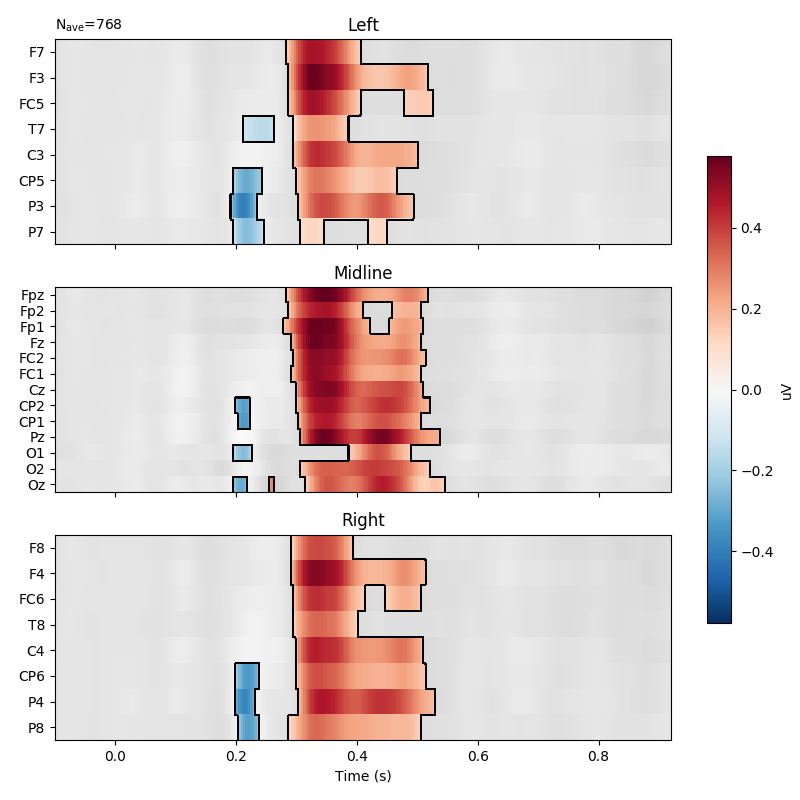
\includegraphics{https://martinos.org/mne/stable/_images/sphx_glr_plot_stats_cluster_erp_002.png}
\caption{image}
\end{figure}


    % Add a bibliography block to the postdoc
    
    
    
    \end{document}
